\documentclass[aspectratio=169]{beamer}
\mode<presentation>{}
\usepackage[utf8]{inputenc}
\newcommand{\fl}[1]{\left\lfloor #1 \right\rfloor}
\newcommand{\fc}[1]{\left\lceil #1 \right\rceil}

\usepackage{multicol}
\usepackage{tikz}
\usepackage{hyperref}

\title{MA 109 : Calculus-I\\ D1 T4, Tutorial 3}
\author{Devansh Jain}
\date[09-12-2020]{9th December 2020}
\institute[IITB]{IIT Bombay}
\usetheme{Warsaw}
\usecolortheme{beetle}
\newtheorem{defn}{Definition}

\begin{document}

\begin{frame}
    \titlepage
\end{frame}

\begin{frame}{Questions to be Discussed}
    \begin{itemize}
        \item Sheet 2
            \begin{itemize}
                \item 8 (ii), (iii) Finding Functions with given Conditions
                \item 10 (i) Sketching curve with given properties
                \item 11 Sketching curve with given properties
            \end{itemize}
        \item Sheet 3
            \begin{itemize}
                \item 1 (ii) Taylor Series for $\arctan x$
                \item 2 Taylor Series for a polynomial
                \item 4 Convergence of Maclaurin Series of $e^x$
                \item 5 Integration using Taylor Series
            \end{itemize}
    \end{itemize}
\end{frame}

\begin{frame}{Tutorial Sheet 2}
    8. (ii). $f''(x) > 0$ for all $x \in \mathbb{R}$, $f'(0) = 1, f'(1) = 2$ \\
    \medskip
    $f''(x) > 0$ for all $x \in \mathbb{R}$ \\
    \medskip
    We know such a curve!!! \\
    \medskip
    Can try quadratic $\implies$ Let $f(x)=ax^2+bx+c$ \\
    $f'(x)=2ax+b$ \hspace{30pt} $f''(x)=2a$ \\
    \medskip
    $f''(x) > 0$  $\implies a>0$ \\
    $f'(0) = 1$ $\implies b=1$ \\
    $f'(1)=2$ $\implies 2a+b=2$ \\
    \medskip
    One such function is: $f(x)=\frac{x^2}{2}+x$ \\
\end{frame}

\begin{frame}{Tutorial Sheet 2}
    8. (iii). $f''(x) \geq 0$ for all $x \in \mathbb{R}$, $f'(0) = 1, f(x) <100$ for all $x>0$ \\
    \medskip 
    \textbf{Idea.}
    Derivative at 0 is positive. \\
    $f''$ non negative, means derivative not decreasing, always positive after 0. \\
    $f$ must be strictly increasing with derivative $>1$, which means, \\
    as x goes to $x+1$, $f(x)$ goes to something $> f(x)+1.$ \\
    (That's what derivative tells us, right?)\\
    But $f(x)$ is bounded above for positive x. Contradiction!!! \\
    \smallskip
    Such a function cannot exist! \\
    Let's write a formal argument. \\
\end{frame}

\begin{frame}{Tutorial Sheet 2}
    8. (iii). \textbf{Proof}. \\
    $f''(x) \geq 0$  \hspace{5pt} $ \forall x \in \mathbb{R} \implies $ $f'$ not decreasing, so $\forall x>0, f'(x)\geq 1$ \\
    To prove: $f$ must exceed 100 at some point. \\
    \medskip
    Can write, using MVT $\dfrac{f(x)-f(0)}{x-0} \geq f'(c) \geq 1$ $\because c \geq 0$ \\
    \smallskip
    Thus, $f(x)\geq x+f(0)$ \\
    \smallskip
    Just take $x=101-f(0) \implies f(x) \geq 101$ . \\
\end{frame}

\begin{frame}{Tutorial Sheet 2}
    10. (i). Graphing the polynomial $f(x)=2x^3+2x^2-2x-1$. \\
    \smallskip
    $f'(x)=6x^2+4x-2 = 2(x+1)(3x-1)$ \\
    \smallskip
    $f'(x)>0$ in $(-\infty, -1) \cup (1/3, \infty)$;  so $f(x)$ is strictly increasing here. \\
    \medskip
    and $f'(x)<0$ in (-1, 1/3) so $f(x)$ is strictly decreasing here. \\
    \medskip
    Thus, $x=-1$ is a local maximum, and $x=\frac{1}{3}$ is a local minimum. \\
    \medskip
    $f''(x)=12x+4$ \\
    \medskip
    Thus, $f(x)$ is concave in $(-\infty,1/3)$ and convex in $(-1/3, \infty)$, \\
    \smallskip
    with a point of inflection at $x=\dfrac{-1}{3}$.
\end{frame}

\begin{frame}{Tutorial Sheet 2}
     10. Graph.\\
    \begin{center}
        \includegraphics[scale=0.24]{desmos-graph.png}
    \end{center}
\end{frame}

\begin{frame}{Tutorial Sheet 2}
    11.
    \begin{figure}
        \centering
        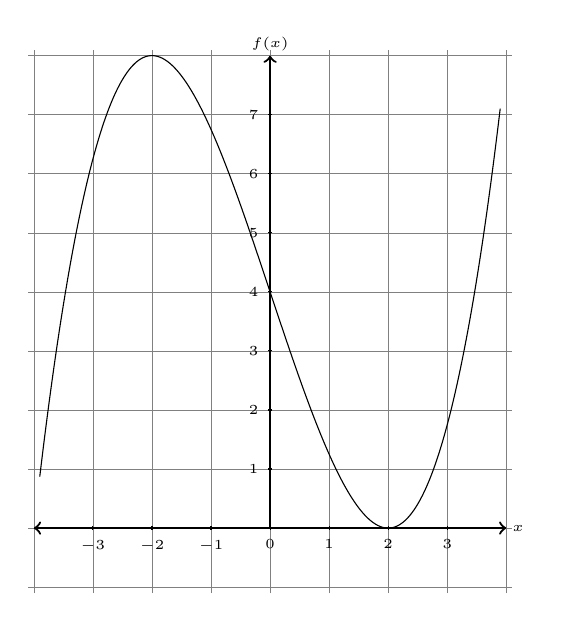
\begin{tikzpicture}[scale = 0.75]
            \draw[step=1cm,gray,very thin] (-4.1,-1.1) grid (4.1,8.1);
            \draw[thick,->] (0,0) -- (4,0);
            \draw[thick,->] (0,0) -- (0, 8);
            \draw[thick,->] (0,0) -- (-4,0);
            \node[] at (4.2, 0) {\tiny $x$};
            \node[] at (0, 8.2) {\tiny $f(x)$};
            \foreach \x in {-3, ..., 3}
                \draw (\x cm,1pt) -- (\x cm,-1pt) node[anchor=north] {\tiny $\x$};
            \foreach \y in {1, ...,7}
                \draw (1pt,\y cm) -- (-1pt,\y cm) node[anchor=east] {\tiny $\y$};
            \draw[variable=\t,domain=-3.9:3.9,samples=500] plot ({\t},{0.25*\t*\t*\t - 3*\t + 4});
        \end{tikzpicture}
    \end{figure}
\end{frame}

\begin{frame}{Tutorial Sheet 2}
	11. (contd.) \\
	I have actually graphed a polynomial that satisfies the given properties. \\
	Can you come up with it? \\
	Is there a unique such polynomial? (We discussed this) \\
	What's the minimum degree of such a polynomial? \\
	Is there a unique polynomial with that degree? (This you should think about)\\
	Suppose you have two distinct polynomials $f$ and $g$ that satisfy the given conditions. Can you come up with a distinct third polynomial such that it satisfies the conditions as well?
\end{frame}

\begin{frame}{Tutorial Sheet 3}
    1. (ii). Taylor Series for arctan x at x=0.  \\
    $\dfrac{d}{dx}(\arctan x)=\dfrac{1}{1+x^2}=g(x)$ (say) \\
    $g(x)=\dfrac{1}{1+x^2}=\displaystyle\sum_{k=0}^\infty (-1)^k x^{2k}$   \\
    (This is only true for $|x|<1$, so we restrict ourselves to that domain.) \\
    \medskip
    $g^{(2k+1)}(0)=0\; $ \hspace{15pt} $g^{(2k)}(0)=(-1)^k (2k)!\; ;\;$ \hspace{5pt} $k\geq 0$ \hspace{5pt} (Do verify this!) \\
    \smallskip
    but these are $n^{th}$ derivatives of $(arctan(x))'$, so are $(n+1)^{th}$ derivatives of $(arctan(x))$. \\
    \medskip 
    Thus the series for arctan x , using the formula $P(x)=\displaystyle \sum_{n=0}^{\infty}\dfrac{f^{(n)}(0)}{n!}(x)^n $ , is : \\
    \smallskip
    $\arctan x= \displaystyle \sum_{n=0}^{\infty} (-1)^n \dfrac{x^{2n+1}}{2n+1}$   \hspace{10pt} (Do verify this!)
\end{frame}

\begin{frame}{Tutorial Sheet 3}
    2. Taylor Series of $f(x)=x^3-3x^2+3x-1 = (x-1)^3$ \\
    Can already guess!!! $f(x)=x^3-3x^2+3x-1$ $\implies f(1)=0$ \\
    \smallskip
    $f'(x)=3x^2-6x+3$ $\implies f'(1)=0$\\
    \smallskip
    $f''(x)=6x-6$   $\implies f''(1)=0$\\
    \smallskip
    $f'''(x)=6$ $\implies f'''(1)=6$\\
    \smallskip
    $f^{(n)}(x)=0$ for all $n>3$.  \\
    \medskip
    The Taylor series is $P(x)=\displaystyle \sum_{n=0}^{\infty}\dfrac{f^{(n)}(x_0)}{n!}(x-x_0)^n$ \\
    Here, only the third derivative is non-zero! Only one term in the Taylor Series! \\
    $P(x)=\dfrac{f'''(0)}{3!}(x-1)^3=\dfrac{6}{6}(x-1)^3=(x-1)^3$
\end{frame}

\begin{frame}{Tutorial Sheet 3}
    4. Proving convergence of the series $\displaystyle \sum_{k=0}^{\infty} \frac{x^k}{k!}$. \\
    \medskip
    We'll follow steps given in the question, i.e. prove Cauchy. \\
    \medskip
    Let us denote the partial sums of of the given series by $s_m(x)$. \\
    We should show that for every $\epsilon>0$, there is a $N \in \mathbb{N}$, such that for all $m, n > N $, $|s_m(x)-s_n(x)|<\epsilon$. \\
    \medskip
    It can be shown that, \\
    for $n>N_0=\fc{2x}+1>2x,$ \hspace{5pt} $\dfrac{x^{n+1}}{(n+1)!} < \dfrac{1}{2}\cdot\dfrac{x^n}{n!}$ (Iteratively, $\dfrac{x^{n+k}}{(n+k)!} < \dfrac{1}{2^k}\cdot\dfrac{x^n}{n!}$) \\
    \medskip
    Observe that (assuming W.L.O.G. $m>n>N_0$), \\
    $\displaystyle |s_m(x)-s_n(x)| = \left|\sum_{k=n+1}^{m} \dfrac{x^k}{k!}\right| \leq \left|\dfrac{x^n}{n!}\right|\left(\dfrac{1}{2} +\dfrac{1}{4} + \dots + \dfrac{1}{2^{m-n}} \right) \leq \dfrac{|x^n|}{n!}$
\end{frame}

\begin{frame}{Tutorial Sheet 3}
    4. (contd.) \\
    We have, \hspace{5pt} $ \displaystyle  |s_m(x)-s_n(x)| \leq \dfrac{|x^n|}{n!} $ for all $m > n$ \\
    Also, by induction, for all $k>0$, we have, \hspace{5pt} $\dfrac{|x|^{N_0+k}}{(N_0+k)!}< \dfrac{1}{2^k} \cdot \dfrac{|x|^{N_0}}{N_0!}$ \\
    \medskip
    For a given $x$ and $\epsilon$, for $N_0=\fc{2x}+1$ choose a $k$ such that $\dfrac{1}{2^k}\cdot \dfrac{|x|^{N_0}}{N_0!} < \epsilon$. \\
    Choose $N=N_0+k$. \\
    Hence this sequence of partial sums of the series $a_n=s_n(x)$ is cauchy for every $x \in \mathbb{R}$ and thus the series is convergent.
\end{frame}

% \begin{frame}{Contractive Sequences}
%     \begin{defn}[Contractive Sequence]
%         A sequence $(a_n), n \in \mathbb{N}$ is contractive iff there exists a constant $c$, with $0\leq    c<1$, such that: \\
%         $|{a_{n+2}-a_{n+1}}|\leqslant{c}\,|{a_{n+1}-a_{n}}|$ for all $n \in \mathbb{N}$
%     \end{defn}
%     Try to prove that a contractive sequence is always cauchy, and thus convergent. \\
%     A Proof is here - \url{http://facstaff.cbu.edu/~wschrein/media/M414\%20Notes/M414L68.pdf} \\
%     \medskip
%     Is the sequence $s_n(x)$ as we defined in the previous question, contractive after $N_0$ terms? \\
%     Does that make the proof easier? Do try this!
% \end{frame}

\begin{frame}{Sheet 3}
    5. To integrate:
    $\displaystyle \int \dfrac{e^x}{x} dx$ \\
    $e^x=\displaystyle \sum_{n=0}^{\infty} \dfrac{x^n}{n!}$  $\implies$  \\
    \smallskip
    $\displaystyle \int \dfrac{e^x}{x} dx =  \displaystyle \int \sum_{n=0}^{\infty} \dfrac{x^{n-1}}{n!}dx$
    $=\displaystyle \int \left( \dfrac{1}{x} + \sum_{n=1}^{\infty} \dfrac{x^{n-1}}{n!}  \right) dx$
    $=\displaystyle \int \dfrac{1}{x} dx + \int \sum_{n=1}^{\infty} \dfrac{x^{n-1}}{n!} dx$ \\
    \medskip
    $=\displaystyle \log(x) + \sum_{n=1}^{\infty} \int  \dfrac{x^{n-1}}{n!} dx$
    $=\displaystyle \log(x) + \sum_{n=1}^{\infty} \dfrac{1}{n!} \dfrac{x^n}{n}$
    $=\displaystyle \log(x) + \sum_{n=1}^{\infty} \dfrac{x^n}{n \cdot n!}$ \\
\end{frame}

\begin{frame}{References}
    Lecture Slides by Prof. Ravi Raghunathan for MA 109 (Autumn 2020) \\
    Tutorial slides prepared by Krushnakant Bhattad for MA 109 (Autumn 2020) \\
    Tutorial slides prepared by Aryaman Maithani for MA 105 (Autumn 2019) \\
    Solutions to tutorial problems for MA 105 (Autumn 2019) \\
\end{frame}

\end{document}
